% Comparison Report: v2 vs v3 vs v4
\documentclass[11pt,a4paper]{article}
\usepackage[utf8]{inputenc}
\usepackage{graphicx}
\usepackage{booktabs}
\usepackage{longtable}
\usepackage{caption}
\usepackage{geometry}
\geometry{margin=1in}
\title{Comparative Evaluation of Waste Prediction Models for Puttalam Solar Salt Production}
\author{Automated report generated from the repository}
\date{\today}

\begin{document}
\maketitle

\begin{abstract}
We compared three candidate waste-prediction models for the Puttalam solar-salt production dataset (2000--2026, 648 samples): the production-grade ensemble \textbf{v2}, and two early prototypes (\textbf{v3} — Ridge multioutput; \textbf{v4} — per-target shallow trees). Using the full dataset for evaluation, \textbf{v2} achieved the highest overall performance (R$^2$ = 0.922; MAE = 13,800; RMSE = 67,247), while \textbf{v4} (R$^2$ = 0.875) and \textbf{v3} (R$^2$ = 0.824) performed less well. The report contains model descriptions, quantitative results, figures and discussion of reasons to adopt \textbf{v2} for production deployment.
\end{abstract}

\section{Models and Methods}
\subsection{v2 (final ensemble)}
Domain-driven feature engineering, per-target learners (gradient boosting, stacking, neural network), OOF stacking and physical post-processing to enforce mass--concentration--volume consistency.

\subsection{v3 (Ridge baseline)}
Compact feature set (production + core weather + month encoding) with a RobustScaler and a MultiOutput Ridge regressor; serves as a fast, interpretable baseline.

\subsection{v4 (per-target shallow trees)}
Per-target DecisionTreeRegressor (max\_depth=4) trained on the same compact features; captures simple non-linearities with low compute cost.

\section{Aggregate results}
Table \ref{tab:agg} summarizes the aggregated metrics computed on the full dataset.

\begin{table}[ht]
\centering
\caption{Aggregated metrics for each model (higher R$^2$ better, lower MAE/RMSE better).}
\label{tab:agg}
\begin{tabular}{lrrr}
\toprule
Model & R$^2$ & MAE & RMSE \\
\midrule
v2 (ensemble) & 0.922254 & 13800.50 & 67246.81 \\
v4 (shallow trees) & 0.874641 & 25302.72 & 113154.57 \\
v3 (Ridge) & 0.824459 & 24114.14 & 109452.66 \\
\bottomrule
\end{tabular}
\end{table}

\section{Per-target R$^2$}
The per-target R$^2$ values (used to produce Figure~\ref{fig:heatmap}) are listed in Table~\ref{tab:per_target}.

\begin{longtable}{lrrr}
\caption{Per-target R$^2$ for each model}\label{tab:per_target}\\
\toprule
Target & v2 & v4 & v3 \\
\midrule
\endfirsthead
\toprule
Target & v2 & v4 & v3 \\
\midrule
\endhead
Total\_Waste\_kg & 0.987219 & 0.961508 & 0.981857 \\
Solid\_Waste\_Gypsum\_kg & 0.991396 & 0.978081 & 0.988021 \\
Solid\_Waste\_Limestone\_kg & 0.991346 & 0.978819 & 0.987905 \\
Solid\_Waste\_Industrial\_Salt\_kg & 0.986256 & 0.896932 & 0.883807 \\
Total\_Solid\_Waste\_kg & 0.997515 & 0.970523 & 0.993684 \\
Liquid\_Waste\_Bittern\_Liters & 0.986268 & 0.961070 & 0.963596 \\
Bittern\_Mg\_Concentration\_gL & 0.840045 & 0.709019 & 0.583059 \\
Bittern\_K\_Concentration\_gL & 0.819670 & 0.700613 & 0.571270 \\
Bittern\_SO4\_Concentration\_gL & 0.850249 & 0.721552 & 0.582074 \\
Bittern\_Ca\_Concentration\_gL & 0.747138 & 0.697502 & 0.565467 \\
Bittern\_Magnesium\_kg & 0.932632 & 0.914855 & 0.860737 \\
Bittern\_Potassium\_kg & 0.928544 & 0.919024 & 0.858051 \\
Bittern\_Sulfate\_kg & 0.935799 & 0.917508 & 0.863215 \\
Bittern\_Calcium\_kg & 0.917482 & 0.917974 & 0.859679 \\
\bottomrule
\end{longtable}

\section{Figures}
\begin{figure}[ht]
\centering
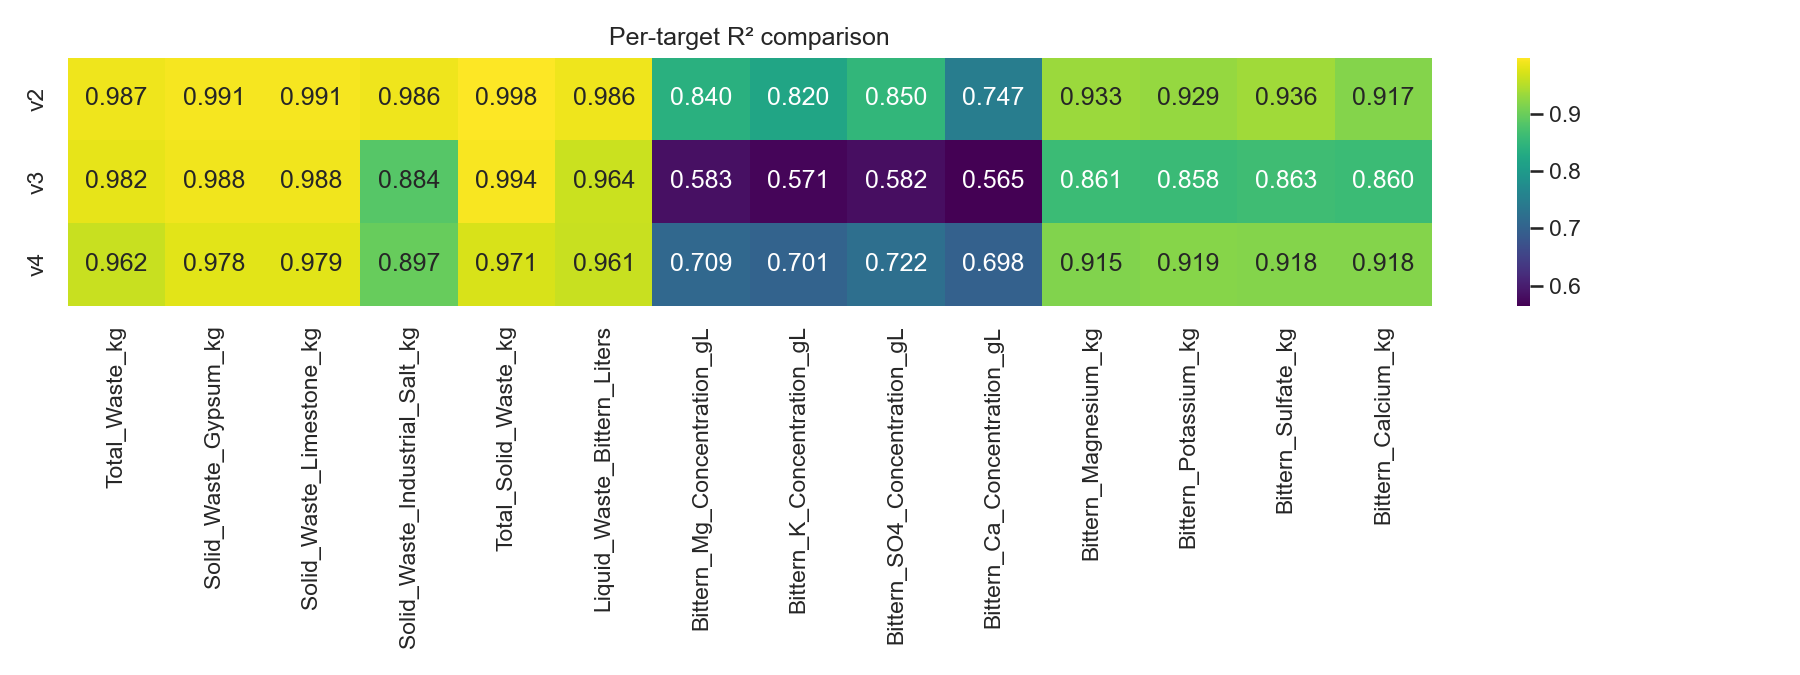
\includegraphics[width=0.95\linewidth]{comparison_plots/per_target_r2_comparison.png}
\caption{Per-target R$^2$ comparison across models (higher is better).}
\label{fig:heatmap}
\end{figure}

\begin{figure}[ht]
\centering
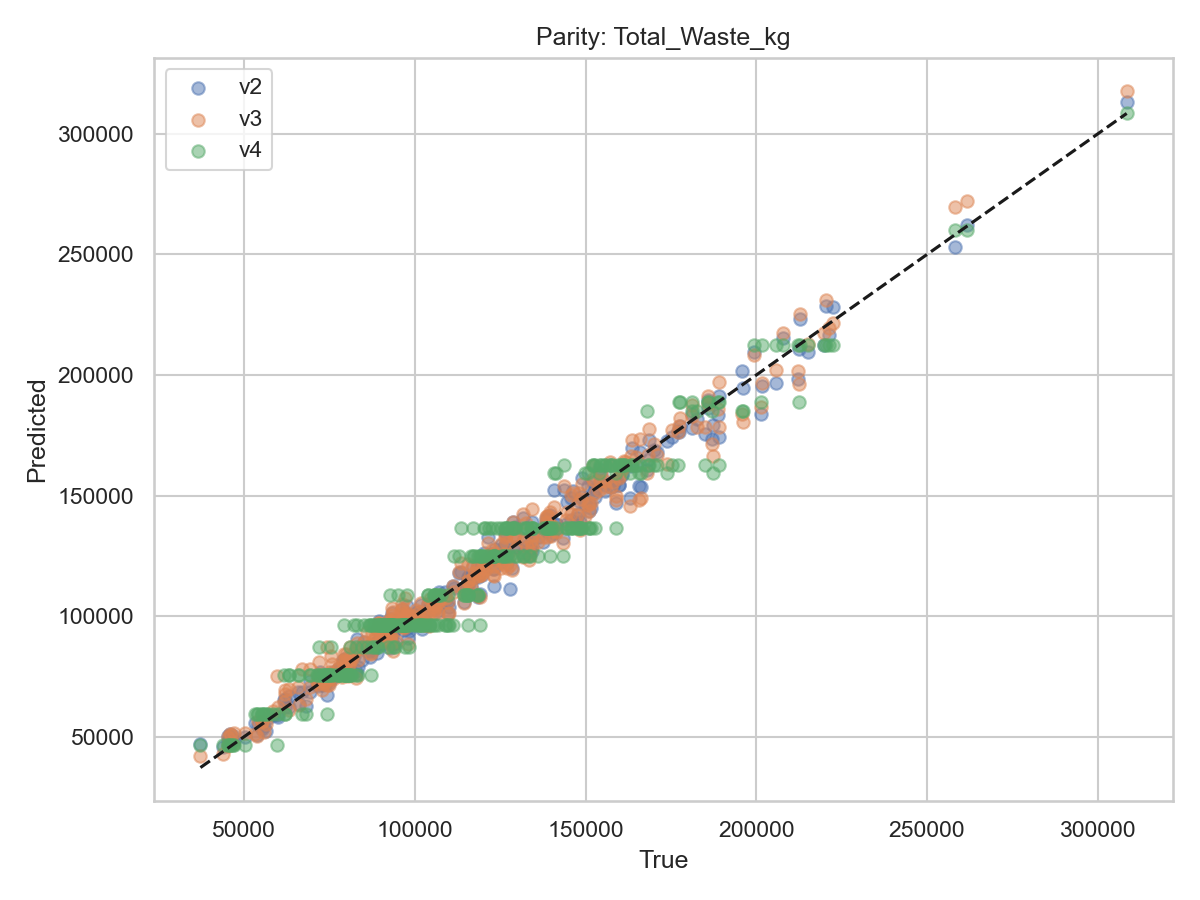
\includegraphics[width=0.8\linewidth]{comparison_plots/parity_Total_Waste_kg.png}
\caption{Parity plot (True vs Predicted) for `Total\_Waste\_kg` across models.}
\label{fig:parity_total}
\end{figure}

\begin{figure}[ht]
\centering
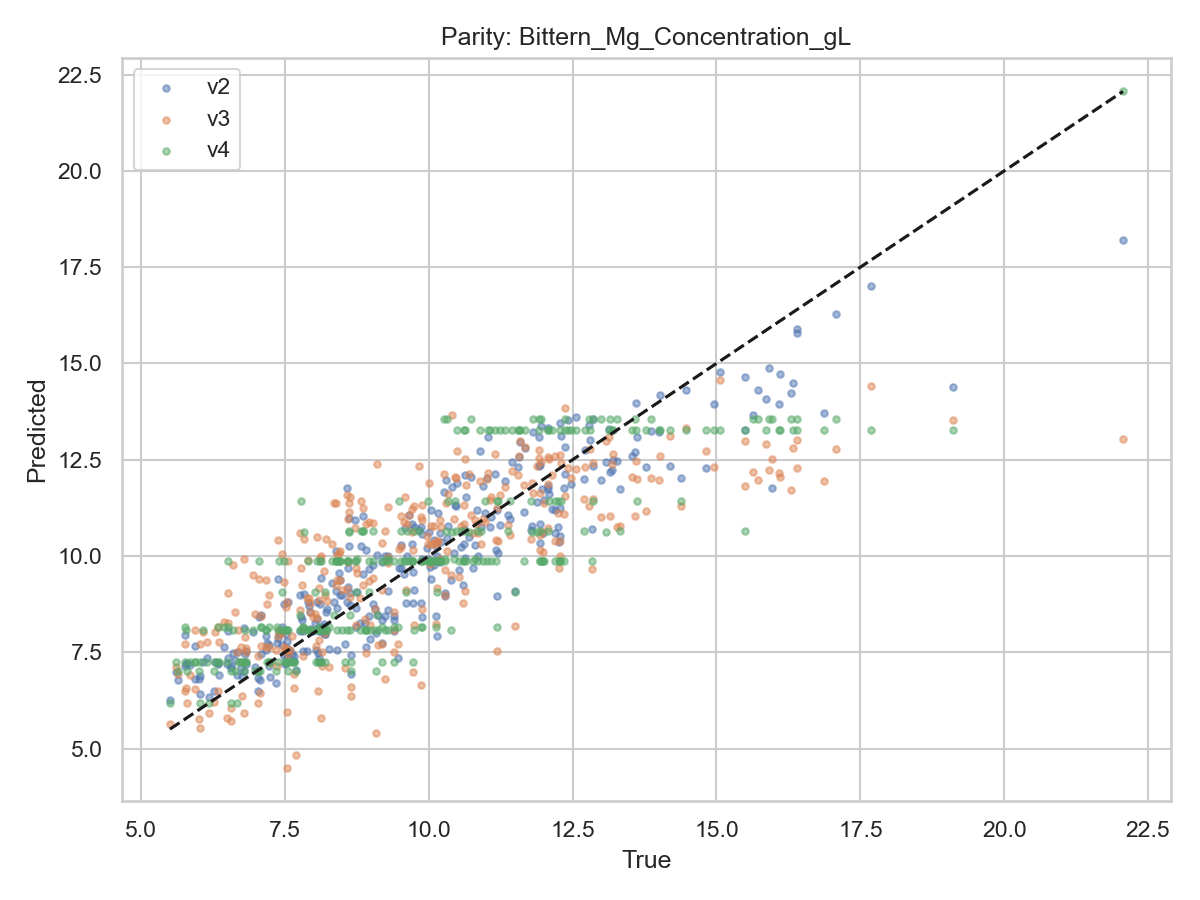
\includegraphics[width=0.8\linewidth]{comparison_plots/parity_Bittern_Mg_Concentration_gL.png}
\caption{Parity plot for `Bittern\_Mg\_Concentration\_gL` (concentration target).}
\label{fig:parity_mg}
\end{figure}

\section{Discussion and rationale for choosing v2}
\begin{itemize}
\item \textbf{Performance:} v2 demonstrates superior aggregate and per-target R$^2$, and substantially lower MAE/RMSE than the simpler baselines.
\item \textbf{Physical plausibility:} v2 applies post-processing to enforce mass-conservation relationships, producing outputs that are more realistic for downstream operational decisions.
\item \textbf{Robustness:} ensemble combination reduces model-specific biases and yields stable per-target performance.
\end{itemize}

\section{Additional materials and reproducibility}
All scripts used to produce these results are in the repository. Run the following in the project root (activated Python environment):
\begin{verbatim}
python v3/train.py
python v4/train.py
python compare_models.py
\end{verbatim}

The main generated artifacts are in the `comparison_plots/` directory: the heatmap and parity plots included above, plus `compare_metrics.json` containing the numeric results.

\section{Notes and possible extensions}
Suggested additional figures (available upon request): residual violin plots per-target; error vs production-volume scatter; calibration plots for concentration targets. These can be generated programmatically if desired.

\end{document}
